\documentclass[11pt]{article}

\usepackage[utf8]{inputenc}
\usepackage{amsmath, amssymb, amsthm}
\newtheoremstyle{mystyle}{}{}{\normalfont}{}{\bfseries}{}{\newline}{}{\bfseries}
\theoremstyle{mystyle}
\newtheorem{problem}{Problem}
\newtheorem*{solution}{Solution}

\usepackage{geometry}
\usepackage{graphicx}
\usepackage{enumitem}
\usepackage{xcolor}
\usepackage{hyperref}
\usepackage{tikz}
\usepackage{fancyhdr}
\usepackage{biblatex}



\geometry{letterpaper, margin=1in}
\pagestyle{fancy}
\fancyhf{}
\rhead{MATH 258A — Spring 2025}
\lhead{Santiago Morales}
\rfoot{Page \thepage}

\title{\vspace{-1cm} \textbf{Homework 6, MAT 258A}}
\author{Santiago Morales \\ UC Davis \\ \texttt{moralesduarte@ucdavis.edu}}
\date{\today}

\begin{document}

\maketitle
\vspace{-1em}
\hrule
\vspace{1em}

\begin{problem}[3]
        For \(C=\{x\in\mathbb{R}^{2}\mid x_{1}+x_{2}=1,\;x_{1}\ge 0,\;x_{2}\ge 0\}\),
        let
        \[
        f(x)=(x_{1}-1)^{2}+x_{2}.
        \]
        Illustrate the contours, and—using the
        Karush--Kuhn--Tucker (KKT) conditions—compute the set of minimisers
        \[
        C_{f}\;:=\;\operatorname*{arg\,min}_{x\in C}f(x).
        \]
        \end{problem}

        


        \begin{solution}

                \begin{solution}
                        We minimize \( f(x) = (x_1 - 1)^2 + x_2 \) over the convex set 
                        \[
                        C = \{ x \in \mathbb{R}^2 \mid x_1 + x_2 = 1,\; x_1 \ge 0,\; x_2 \ge 0 \}.
                        \]
                        The Lagrangian is:
                        \[
                        \mathcal{L}(x_1, x_2, \lambda, \mu_1, \mu_2) = (x_1 - 1)^2 + x_2 - \lambda(x_1 + x_2 - 1) - \mu_1 x_1 - \mu_2 x_2,
                        \]
                        with KKT conditions:
                        \[
                        \begin{cases}
                        2(x_1 - 1) - \lambda - \mu_1 = 0, \\
                        1 - \lambda - \mu_2 = 0, \\
                        x_1 + x_2 = 1,\quad x_1, x_2 \ge 0, \\
                        \mu_1 x_1 = 0,\quad \mu_2 x_2 = 0,\quad \mu_1, \mu_2 \ge 0.
                        \end{cases}
                        \]
                        
                        Case 1: \( x_2 = 0 \Rightarrow x_1 = 1 \). Then \( \mu_2 \cdot 0 = 0 \), and from the stationarity conditions:
                        \[
                        2(1 - 1) - \lambda - \mu_1 = 0 \Rightarrow \lambda = -\mu_1, \quad 1 - \lambda - \mu_2 = 0.
                        \]
                        Setting \( \mu_1 = 0 \Rightarrow \lambda = 0,\; \mu_2 = 1 \). All KKT conditions are satisfied.
                        
                        Other cases (e.g., \( x_1 = 0 \)) lead to higher objective values. Therefore, the unique minimizer is
                        \[
                        C_f = \{ (1, 0) \}.
                        \]
                        \end{solution}
% add subgrad.png
\begin{center}
        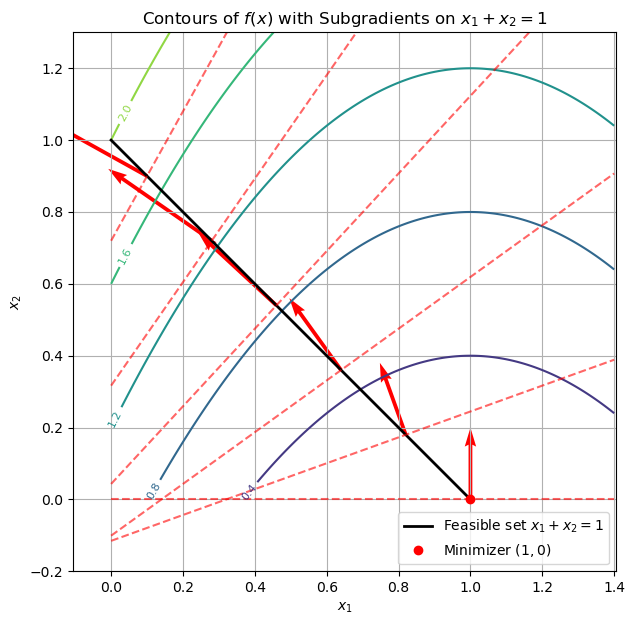
\includegraphics[width=0.5\textwidth]{subgrad.png}
        \end{center}
        \end{solution}



    
\end{document}